\section{Preposition}

Prepositions\index{preposition} also are not an independent POS. They are closely related to the main word (often it is a noun). Most prepositions show the direction or the location of the action. 

We can divide prepositions into two main groups, so as we did with adverbs. We can distinguish \textit{primary} and \textit{secondary} prepositions. Primary prepositions are very ancient and we cannot refer to any word form they have formed from. Secondary prepositions are longer, and they appeared by semantic shift of an adverb, transgressive or a cased-noun. 

Here I will list primary prepositions with English translations and controlled cases. Complex cases are commented in notes.

\textit{Bez} (Gen.) - Without

\textit{V} (Acc.) - In, into

\textit{Dlä} (Gen) - For

\textit{Do} (Gen.) - To

\textit{Za} (Instr.) - For

\textit{Iz} (Gen.) - From (inside the object)

\textit{K} (Dat.) - To

\textit{Krôz} (Skrôz) (Gen.) - Through

\textit{Na} (Acc.) - On

\textit{Nad} (Instr.) - Above

\textit{O} (Prep.) - About

\textit{Od} (Gen.) - From (the object)

\textit{Po} (Dat.) - Along

\textit{Pod} (Instr.) - Under

\textit{Pri} (Loc.) - At

\textit{Pro} (Acc.) - About (the difference between “O” and “Pro” is in the detail view on the object. When we say the second variant we just mention the object in our speech, while using the first one we talk about it in details).

\textit{S} (Instr.) - With

\textit{U} (Gen.) - At (the difference between “Pri” and “U” is in the object of speaking. When we use “U” we mention real object in space and place the object of speaking near it. “Pri” is used when we speak about proximity in time, i.e. some events are close to each other.)

\textit{Črez} (Acc.) - After,  in (time)

The following figure shows the semantics of most primary prepositions.

\begin{figure}
	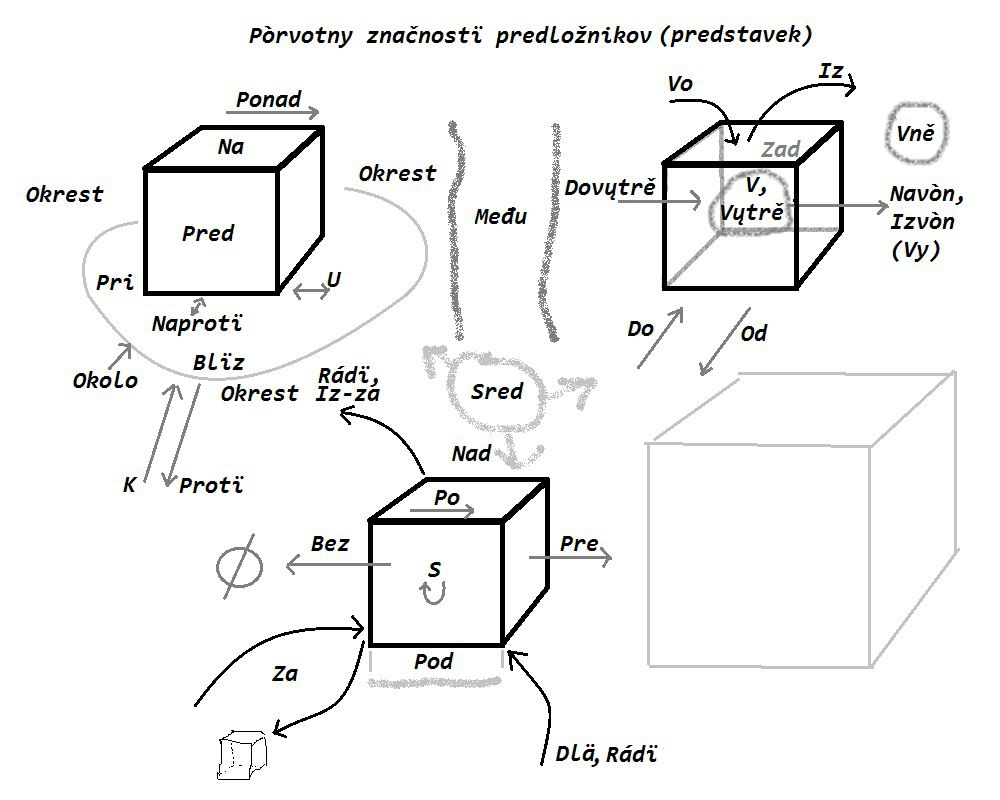
\includegraphics[width=\linewidth]{./sources/prepositions.jpeg}
	\caption{Prepositions in Novoslovnica}
	\label{fig:prepositions}
\end{figure}

Secondary prepositions are derived from nouns or adverbs with the shift of semantic from independent to an auxiliary one. For examples, preposition "Pred" is derived from the noun "Pred" (Front). Using separately in refers to a frontal part of something. Using with an additional independent word it becomes a preposition defining the frontal part of the word that follows it.

\textbf{Examples:}

\textit{Svòrh} - Over

\textit{Među} - Between